
\begin{figure}[H]
	\center
	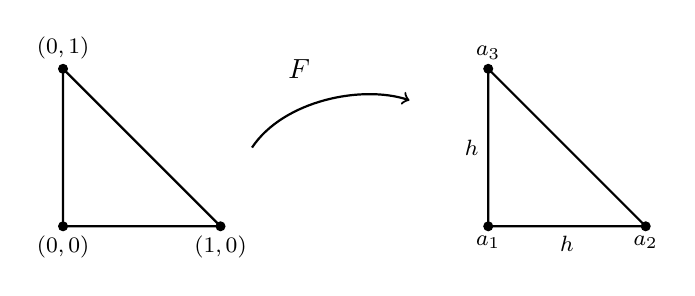
\begin{tikzpicture}[scale=2]
	
	
	% first simplex
	\draw[thick] (0,0) -- ++(0,1) -- ++(1,-1)--cycle;
	\filldraw (0,0)         circle (0.8pt)
			  (0,0) ++(1,0) circle (0.8pt)
			  (0,0) ++(0,1) circle (0.8pt);
	\fill[black,font=\footnotesize] (0,0) node[below] {$(0,0)$}
									(0,0) ++(1,0) node[below] {$(1,0)$}
									(0,0) ++(0,1) node[above] {$(0,1)$};
	
	%arrow
	\draw[thick,-to] (1.2,0.5) .. controls (1.4,0.8) and (1.9,0.9) .. (2.2, 0.8);
	
	%second simplex							
	\draw[thick] (0,0) ++ (2.7,0) -- ++(0,1) -- ++(1,-1)--cycle;
	\filldraw 	(0,0) ++ (2.7,0)         circle (0.8pt)
				(0,0) ++ (2.7,0) ++(1,0) circle (0.8pt)
				(0,0) ++ (2.7,0) ++(0,1) circle (0.8pt);
	%\filldraw (2.2,0)         circle (0.8pt)
	%		  (2.2,0) ++(2,0) circle (0.8pt)
	%		  (2.2,0) ++(1,1) circle (0.8pt);
	\fill[black,font=\footnotesize] (2.7,0) node[below] {$a_1$}
									(2.7,0) ++(1,0) node[below] {$a_2$}
									(2.7,0) ++(0,1) node[above] {$a_3$};								
			
	
	
	%\draw (2.2,0) ++(45:.6) arc (45:0:.6);
	
	
	\node at (1.5,1) {$F$};
	\fill[black,font=\footnotesize] (3.2,0)  node[below] {$h$}
									(2.7,0.5) node[left] {$h$};
	\end{tikzpicture}
	
	\caption{$F:\hat{\tau} \to \tau $}
	\label{ch2_plot_f}
	
\end{figure}